\documentclass[letterpaper,man,natbib]{apa6}
\usepackage[english]{babel}
\usepackage[utf8x]{inputenc}
\usepackage{amsmath}

\usepackage{graphicx}
\usepackage{float}
\usepackage{caption}
\usepackage{subcaption}
\captionsetup{justification=centering}

\usepackage{url}
\def\UrlBreaks{\do\/\do-}
\usepackage{breakurl}


\pagenumbering{gobble}

%
%%Below is what you can edit
\title{}  % TODO
\shorttitle{}
\author{Tziporah Horowitz}
\affiliation{Johns Hopkins University}

\abstract{Your abstract here.}  % TODO

\begin{document}
%\maketitle


\section{Introduction}\label{sec:introduction}

\pagebreak

\section{Methods}\label{sec:methods}

\begin{minipage}{.9\linewidth}
 \usepackage[english]{babel}
\usepackage[utf8x]{inputenc}
\usepackage{amsmath}

\usepackage{graphicx}
\usepackage{float}
\usepackage{caption}
\usepackage{subcaption}
\captionsetup{justification=centering}

\usepackage{url}
\def\UrlBreaks{\do\/\do-}
\usepackage{breakurl}


\begin{float}
     \centering
     \begin{subfigure}[b]{0.32\textwidth}
         \centering
         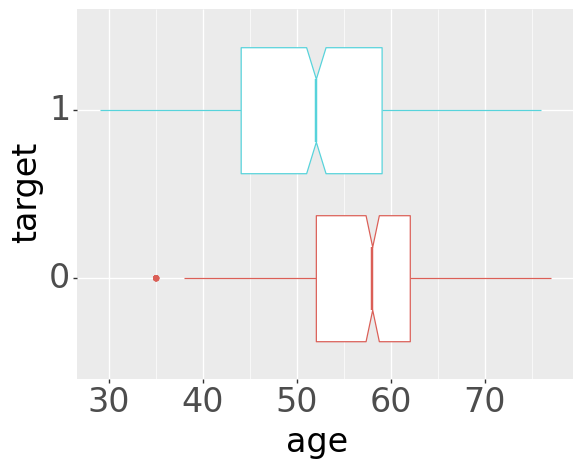
\includegraphics[width=\textwidth]{plots/target-age.png}
     \end{subfigure}
     \begin{subfigure}[b]{0.32\textwidth}
         \centering
         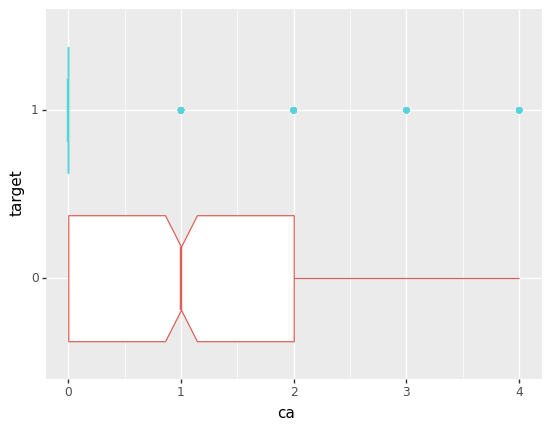
\includegraphics[width=\textwidth]{plots/target-ca.png}
     \end{subfigure}
     \begin{subfigure}[b]{0.32\textwidth}
         \centering
         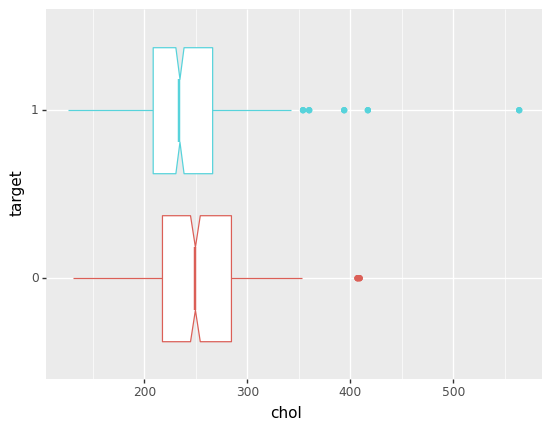
\includegraphics[width=\textwidth]{plots/target-chol.png}
     \end{subfigure}

     \begin{subfigure}[b]{0.32\textwidth}
         \centering
         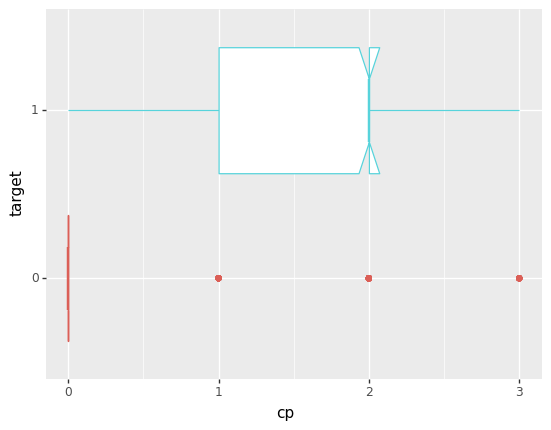
\includegraphics[width=\textwidth]{plots/target-cp.png}
     \end{subfigure}
     \begin{subfigure}[b]{0.32\textwidth}
         \centering
         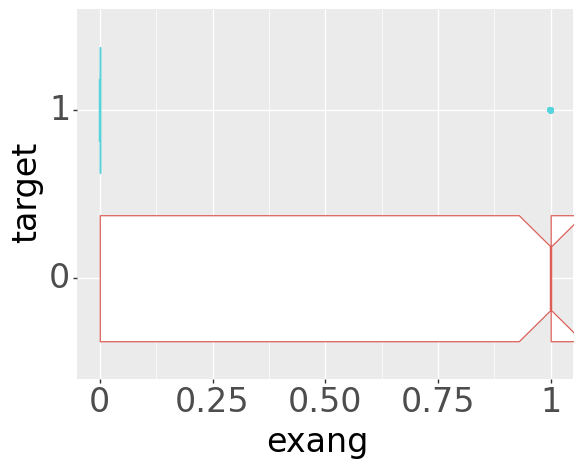
\includegraphics[width=\textwidth]{plots/target-exang.png}
     \end{subfigure}
     \begin{subfigure}[b]{0.32\textwidth}
         \centering
         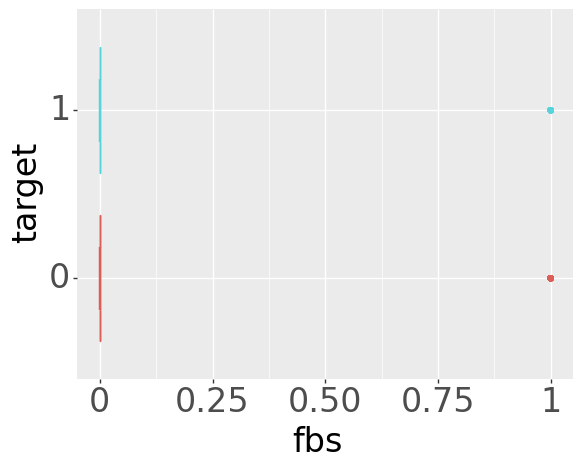
\includegraphics[width=\textwidth]{plots/target-fbs.png}
     \end{subfigure}

     \begin{subfigure}[b]{0.32\textwidth}
         \centering
         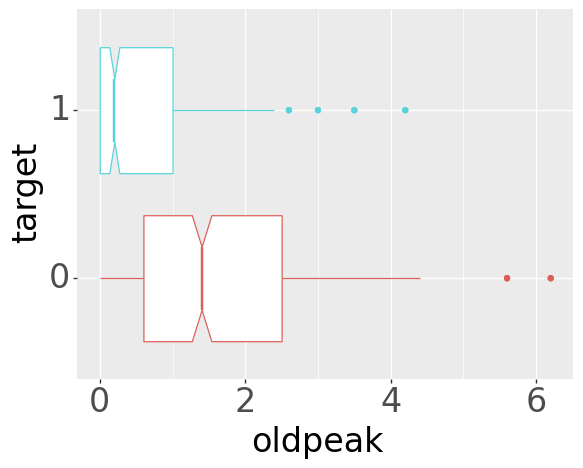
\includegraphics[width=\textwidth]{plots/target-oldpeak.png}
     \end{subfigure}
     \begin{subfigure}[b]{0.32\textwidth}
         \centering
         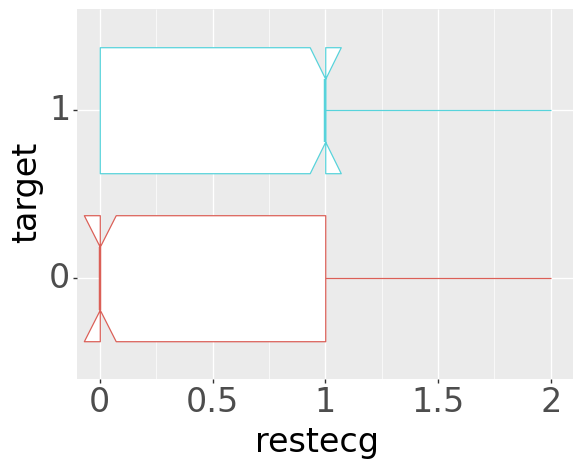
\includegraphics[width=\textwidth]{plots/target-restecg.png}
     \end{subfigure}
     \begin{subfigure}[b]{0.32\textwidth}
         \centering
         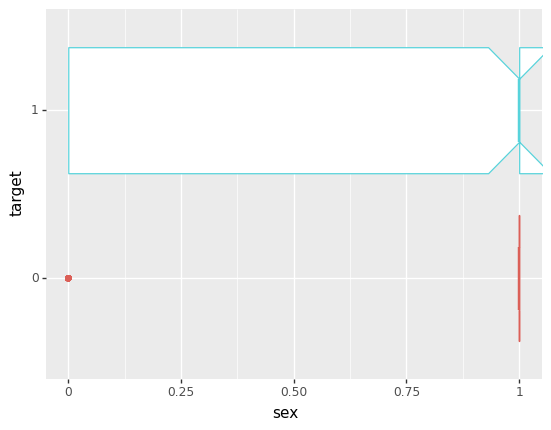
\includegraphics[width=\textwidth]{plots/target-sex.png}
     \end{subfigure}

     \begin{subfigure}[b]{0.32\textwidth}
         \centering
         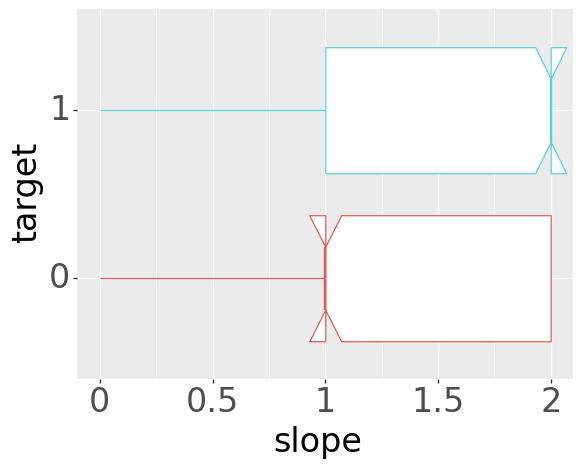
\includegraphics[width=\textwidth]{plots/target-slope.png}
     \end{subfigure}
     \begin{subfigure}[b]{0.32\textwidth}
         \centering
         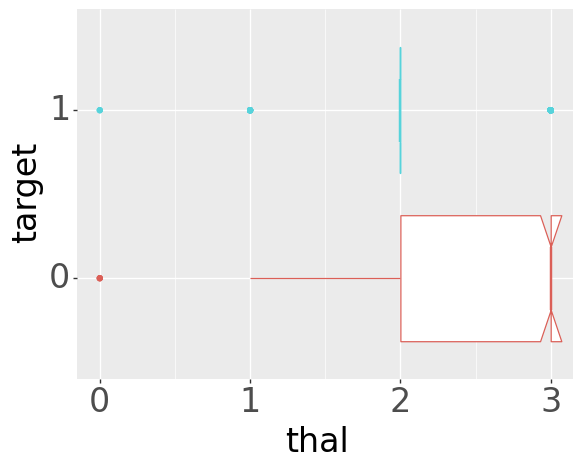
\includegraphics[width=\textwidth]{plots/target-thal.png}
     \end{subfigure}
     \begin{subfigure}[b]{0.32\textwidth}
         \centering
         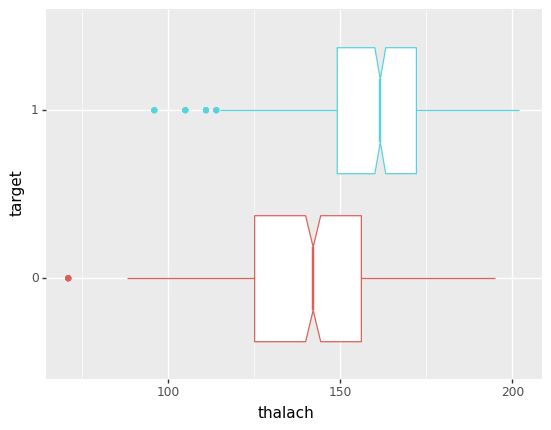
\includegraphics[width=\textwidth]{plots/target-thalach.png}
     \end{subfigure}

     \begin{subfigure}[b]{0.32\textwidth}
         \centering
         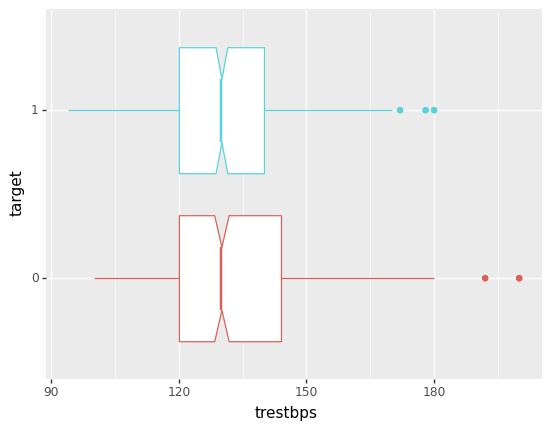
\includegraphics[width=\textwidth]{plots/target-trestbps.png}
     \end{subfigure}

     \caption[Figure]{Distributions of Independent Variables} \label{fig:subdistributions}
\end{float}
 \captionof{figure}{Distributions of Features}
\end{minipage}


\subsection{This is a Subsection}\label{subsec:this-is-a-subsection}
% \cite{Marginal-Effects—Quantifying-the-Effect-of-Changes-in-Risk-Factors-in-Logistic-Regression-Models}
% \cite{Relative-Measures-of-Association-for-Binary-Outcomes:-Challenges-and-Recommendations-for-the-Global-Health-Researcher-ue}
% \cite{Log-Odds-and-the-Interpretation-of-Logit-Models}
% \cite{Statistical-hypothesis-testing}
% \cite{An-Introduction-to-Logistic-Regression-Analysis-and-Reporting}
% \cite{Problems-with-Using-Odds-Ratios-as-Effect-Sizes-in-Binary-Logistic-Regression-and-Alternative-Approaches}
% \cite{Using-Logistic-Regression-Model-to-Study-the-Most-Important-Factors-Which-Affects-Diabetes-for-The-Elderly-in-The-City-of-Hilla}


\pagebreak

\bibliography{main}

\end{document}

